\chapter{Background} \label{ch:background}

Detailed description of many things. Blurb - brief description of cheminformatics, applications of computational tools to drug discovery. Maybe introduce design-make-teset? This stuff is probably in the introduction.

\section{Molecular Representation}

\subsection{SMILES}
The simplified molecular-input line-entry system (SMILES) \cite{Weininger1988, Weininger1989} is a widely-used text-based description of molecular structure. In SMILES strings, atoms are represented with their chemical symbols and aromatic atoms are denoted in lowercase. Single and aromatic bonds are omitted while for double and triple bonds the specials characters \texttt{=} and \texttt{\#} are used. Branches are specified by enclosing them into parentheses. To encode cyclic structures a single bond in the ring is broken and the matching atoms are denoted by numbers. \texttt{@} characters are used to denote chirality while \texttt{\textbackslash} and \texttt{/} characters specify local double bond configurations. Following these rules, a SMILES string is constructed by traversing the nodes of the molecular graph. Depending on the choice of starting node and traversal route there are often multiple valid SMILES representations per molecule, especially for larger molecules. In order to define a single unique SMILES representation for a molecule, known as the `canonical' SMILES, a deterministic algorithm is used to choose the starting node and traversal route.

(Table~\ref{table:smiles})
\begin{table}[!h]
\begin{center}
    \begin{tabular}{|c|c|}
    \hline
         SMILES & Structure \\
         \hline
         C & CH\textsubscript{4} \\
         \lbrack Fe2+\rbrack & Fe\textsuperscript{2+} \\
         C=O & CH\textsubscript{2}O \\
         C\#N & HCN (cyan) \\
         CCN(CC)CC & 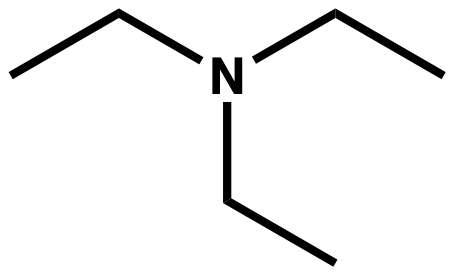
\includegraphics[width=0.75in]{Chapters/Background/Figs/triethyl_amine.png} \\
         CC1=CC(CCC1)Br & 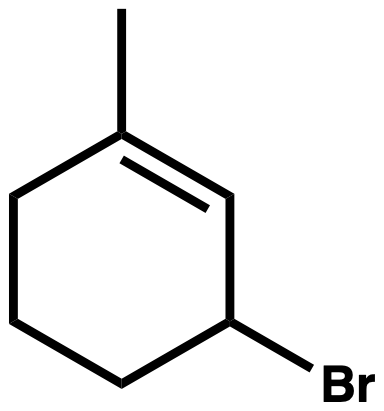
\includegraphics[width=0.7in]{Chapters/Background/Figs/cyclic.png} \\
         \hline
    \end{tabular}
    \caption{Demonstration of the SMILES language}
    \label{table:smiles}
\end{center}
\end{table}

Reaction SMILES are a simple extension of SMILES for specifying chemical reactions. Reaction SMILES strings constructed by placing a \texttt{>} character between the SMILES strings of reactants, reagents, and products. If multiple molecules participate in the reactio, their SMILES strings are separated by a period (\texttt{.}) character.

The text-based nature of SMILES strings as well as its expressiveness in encoding the molecular graph alongside stereochemistry results in its widespread use for storing chemical data. In the context of machine learning, the vast majority of molecular datasets where ML models are used will have molecules represented as SMILES strings. For example, the (blah blah) dataset consists of (blah) SMILES strings alongside the measured (blah) value for each molecule, while USPTO consists of (blah) reaction SMILES strings. For text-based ML models such as the Molecular Transformer (see chapter \ref{ch:transformer}), the SMILES strings are directly input to the model, while for other types of models the SMILES strings will be further processed to generate the necessary input features.

\begin{figure}[!h]
    \centering
    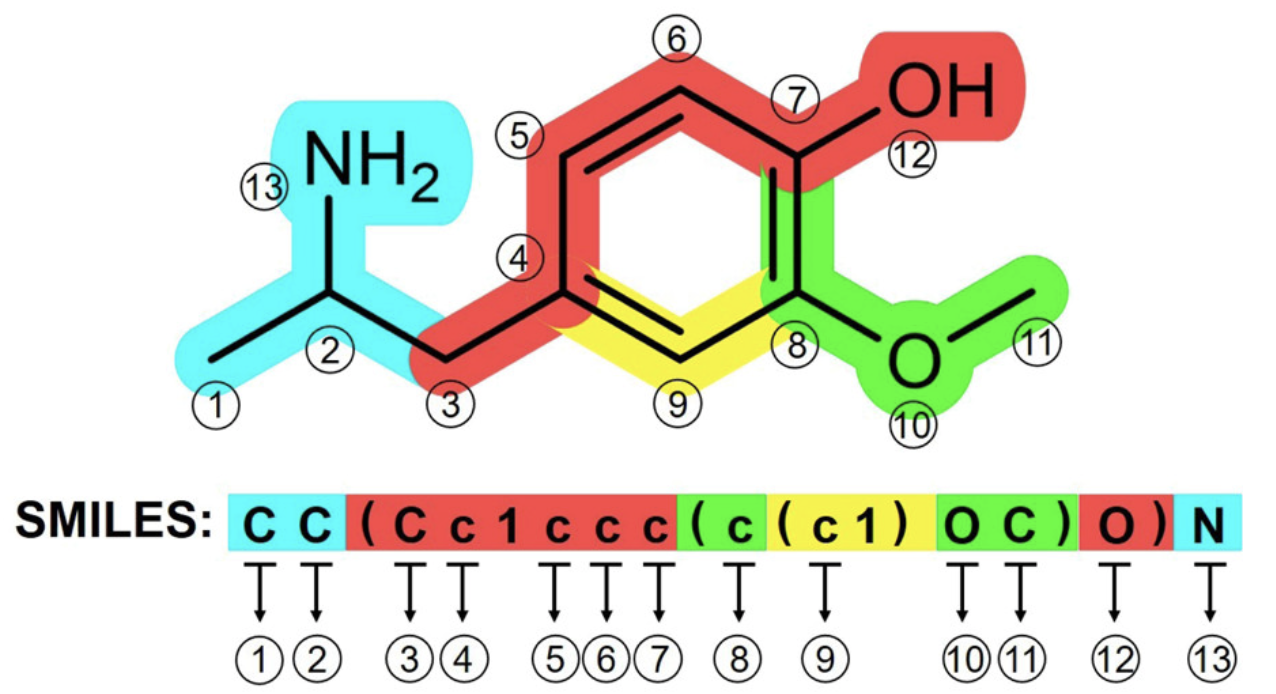
\includegraphics[width=0.8\textwidth]{Chapters/Background/Figs/smiles.png}
    \caption{\label{fig:smiles} \textbf{Illustration of the mapping from chemical structure to SMILES.} Adapted from \cite{Kim2021GenerativeCT}.}
\end{figure}

While SMILES is by far the most widely used text-based representation of molecules, other representations have been developed and are in use to address some shortcomings in SMILES. For example, the International Chemical Identifier (InChI) \cite{Heller2013InChI} string representation, which has a hierarchical construction for specifying tautomeric/stereochemical/charge states, allows greater precision and flexibility in querying molecules from large chemical databases. Another example is SELF-referencIng Embedded Strings (SELFIES) \cite{Krenn2020Selfies} which is constructed such that every SELFIES string, including random combinations of characters, is a valid molecule. This property is useful for the application of ML models that generate text as output - using SELFIES as the molecular representation, the model always output valid molecules whereas with SMILES that is not guaranteed.

\subsection{SMARTS} \label{subsec:smarts}
Given a dataset of molecules or chemical reactions encoded with SMILES, we often want to identify molecules or reactions that contain a specific substructure. For example, we may want to identify molecules that contain a specific functional group or reaction that contains a specific reaction center. The standard tool for performing these substructure queries is via SMILES Arbitrary Target Specification (SMARTS) notation. The SMARTS line notation is expressive and allows extremely precise and transparent substructural specification and atom typing.

Using many of the same symbols as SMILES, it also allows specification of wildcard atoms and bonds, which allows expressive and precise definitons of substructures and atomic environments for searching chemical databases. One common misconception is that SMARTS-based substructural searching involves matching of SMILES and SMARTS strings. When performing a SMARTS query on a SMILES string, both SMILES and SMARTS strings are first converted to internal graph representations which are then searched for subgraph isomorphism.

\begin{table}[!h]
\begin{center}
    \begin{tabular}{|c|c|}
    \hline
        SMARTS & Substructure \\
        \hline
        [C;R] &  An aliphatic carbon in a ring \\\relax
        [\#6]@[\#6] & Two carbons connected by a ring bond \\\relax
        [N;\$(NC=[O,S])] & amide or thioamide nitrogen \\\relax
        [N:1][C:2](=[O:3])[N:4]>>[N:1][C:2](=[O:3])[C:4] & urea group transforming into an amide \\
        \hline
    \end{tabular}
    \caption{Examples of SMARTS patterns}
    \label{table:smarts}
\end{center}
\end{table}
%  C\#N & recursive \\

The precise substructure specification of SMARTS is useful in many aspects in the drug design process. For example, a common step in assessing the quality of a proposed drug candidate is to perform a SMARTS query to identify if the hit contains any substructures that are likely to produce artifacts in biochemical or cellular assays. These substructures are typically functional groups with a marked propensity to bind to multiple targets, so-called nuisance compounds, which are of little value in drug discovery. Many different sets of these filters have been compiled in the literature such as REOS (rapid elimination of swill) \cite{Walters1998overview} and PAINS (Pan Assay Interference Compounds) Filters \cite{Baell2010Pains}. Similarly, SMARTS queries are used to design `structural alerts' which flag molecules containing reaction chemical substructures which may lead to undesirable toxicity in the compound itself or its metabolites \cite{Limban2018StrucuralAlerts}.

Another use of SMARTS is in the labelling of pharmacophores in a molecule. Pharmacophores are an abstract description of the molecular features involved in ligand binding - typical examples of such features are hydrogen bond acceptors/donors and aromatic rings. SMARTS strings are used to map different molecular substructures to particular pharmacophore features and then to query for the presence of these features in a molecule. As with substructure filtering, different companies in the pharmaceutical industry have different/propritary sets of SMARTS strings tailored for their particular use cases. (see section \ref{subsec:pharmacophores} for details)

Beyond substructures for individual molecules, SMARTS can also be applied to reaction SMILES to capture transformation in substructures. These SMARTS strings for chemical reactions are often referred to in the literature as `reaction templates'. For example... Beyond querrying for matching reactions from a dataset, reaction templates can also be directly applied to a set of molecules to computationally generate a `reaction product'. This approach is used to generate virtual libraries \textit{in silico}eg EnamineREAL.

% Often it is not necessary to fully simulate and understand a chemical reaction and it is sufficient to know the outcome i.e. the major product of it. This is most often the case when experimental organic chemists are willing to validate their synthetic route or when a synthesis planning software uses a reaction prediction model to score its suggestions. This is what is more traditionally referred to as reaction prediction. In these use cases a general purpose model that is able to predict a wide variety of organic reactions with good accuracy is desired. Trained organic chemists usually rationalize reactions based on the reaction mechanisms \cite{Clayden2012}. These mechanisms can be used to categorize organic reactions and each of these categories can be summarised with the help of so called reaction templates. Figure~\ref{fig:rx_template} shows a typical general reaction template for the synthesis of an amide using acid chloride and an amine. Here the $R_1$ and $R_2$ represent any chemical structures.

\begin{figure}[htbp!] 
    \centering    
    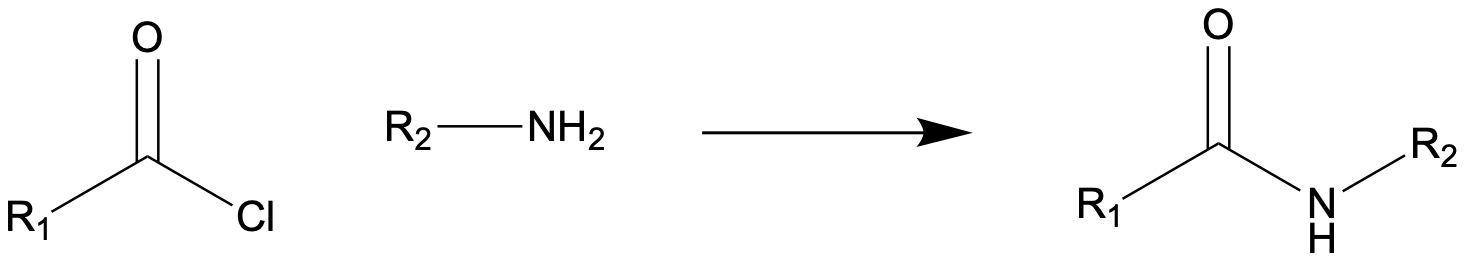
\includegraphics[width=0.75\textwidth]{Chapters/Background/Figs/rx_template.png}
    \caption[Reaction template]{An example of a reaction template for the synthesis of an amide}
    \label{fig:rx_template}
\end{figure}

In addition to virtual library construction, reaction templates can be used for organic reaction prediction by first building a catalogue of possible reaction templates. Then given some reactants and reagents as labelled graphs the problem of reaction prediction is transformed into one of subgraph searching to find the best matching general template in the catalogue. When that template is found it can be applied on the input to obtain the predicted outcome of the reaction. This approach was originally proposed and pioneered in the 1980s for the reverse problem of retrosynthesis \cite{Corey1985ComputerAssistedSynthesis}. The template-based approach had some success in forward reaction prediction for example as described in Ref~\cite{Klucznik2018EfficientLaboratory} a template-based model helped design synthetic pathways to a diverse set of 8 drug-like molecules. This method had considerably more success in retrosynthesis though where there does not exist a single correct solution. One of the major limitation of template-based approaches when applied to forward prediction is scalability, meaning that the template library needs to be maintained and every time a new reaction is reported the associated template needs to be added to the template library. A further problem is that it is often not obvious which parts of the molecule are crucial for a given reaction. This means that given a reaction one can derive a smaller more general template or a larger one that is more specific for the particular reaction. This results in either too many templates matching a particular input resulting in many equally possible reaction outcomes or in the case of larger more specific templates the library will grow very big which results in very slow predictions.

\subsection{Pharmacophores} \label{subsec:pharmacophores}

A pharmacophore is an abstract description of molecular features that are necessary for molecular recognition of a ligand by a biological macromolecule \cite{Kaserer2015PharmacophoreReview}. IUPAC defines a pharmacophore to be "an ensemble of steric and electronic features that is necessary to ensure the optimal supramolecular interactions with a specific biological target and to trigger (or block) its biological response".[1] A pharmacophore model explains how structurally diverse ligands can bind to a common receptor site. Furthermore, pharmacophore models can be used to identify through de novo design or virtual screening novel ligands that will bind to the same receptor.

Typical pharmacophore features include hydrophobic centroids, aromatic rings, hydrogen bond acceptors or donors, cations, and anions. These pharmacophoric points may be located on the ligand itself or may be projected points presumed to be located in the receptor.

In modern computational chemistry, pharmacophores are used to define the essential features of one or more molecules with the same biological activity. A database of diverse chemical compounds can then be searched for more molecules which share the same features arranged in the same relative orientation. Pharmacophores are also used as the starting point for developing 3D-QSAR models. Such tools and a related concept of "privileged structures", which are "defined as molecular frameworks which are able of providing useful ligands for more than one type of receptor or enzyme target by judicious structural modifications",[3] aid in drug discovery.[4]

Pharmacophore models can be generated using two different approaches (Figure 2) depending on the input data employed for model construction. In the structure-based approach, the interaction pattern of a molecule and its targets are directly extracted from experimentally determined ligand-target complexes (Figure 2A). An important source for these complexes, e.g., derived from NMR-spectroscopy or X-ray crystallography, represents the Protein Data Bank (PDB, www.pdb.org) [9]. To date (access date 2 November 2015), more than 113,000 macromolecular structures are stored in this online repository. However, not all of these structures were solved in a complex with a bound ligand, and in the case of induced fit, the binding of different ligands to an enzyme or receptor can lead to different interactions that are not covered by a single structure. To address this limitation, some pharmacophore modeling programs, e.g., Discovery Studio [7] and LigandScout [6], also provide tools to create pharmacophore models based exclusively on the topology of the binding site and in the absence of a ligand [10]. In Discovery Studio, for example, the binding site can be defined manually by selecting residues within the desired cavity or by applying implemented binding site identification tools. Once the binding site is defined, the program automatically calculates pharmacophore features based on the residues lining the active site. This initial ensemble of pharmacophore features can then be adapted to construct the final hypothesis [10]. In addition, structure-based pharmacophore models can also be generated with computationally derived ligand-target complexes. In the course of a docking run, known active compounds are fitted into the empty binding pocket of the target [11]. These docked binding poses can then directly be employed to extract the interaction patterns. For further refinement of the initial docking poses, molecular dynamics (MD) simulations can be conducted [12] prior to model generation.
In the course of ligand-based modeling, three-dimensional (3D) structures of two or more known active molecules are aligned and common pharmacophore features shared among these training set molecules are identified (Figure 2B). In a ligand-based approach, all of the common chemical features from the pharmacophore have to be presumed as essential, whereas in a structure-based approach, it can be considered whether a chemical feature of a molecule is directly involved in the ligand binding or not.

Use SMARTS to define pharmacophores.

\subsection{Fingerprints} \label{subsec:fingerprints}

In order to apply powerful machine learning methods, we require a (typically fixed-length) vector representation of molecules konwn in the literature as `molecular fingerprints'. The most popular molecular fingerprint is the Morgan fingerprint \cite{morgan1965fingerprints}, also known as the Extended-Connectivity FingerPrint (ECFP) \cite{rogers2010extended}. ECFPs are a particular example of `topological' fingerprints that encode the presence of substructures in a molecule by traversing the molecular graph.

ECFPs are generated via a recursive hashing algorithm that numerically hashes the representation of each atom with those of its neighbours, and again with it's next-nearest neighbours etc until a pre-defined `radius' is reached. The resulting hash values are then used to generate a fixed-length binary vector of 1/0 bits. The length of the vector is pre-determined and each 1-bit represents a unique substructure that is encountered during the traversal. The radius of the graph traversal is also a pre-defined parameter that controls the size of the substructures that are represented in the fingerprint. The radius is typically set to 2 or 3, and the length of the fingerprint is typically in the range of 1024-4096.

The popularity of the Morgan fingerprint owes to its usefullness in calculating molecular similarity \cite{Maggiora2014similarity}. Intuitively, we would expect two molecules that have `similar' molecular fingerprints to have similar chemical structures. Numerically, we can quantify the similarity between two molecular fingerprints by the Tanimoto coefficient \cite{Willet1998similarity}:

\begin{equation} \label{eqn:tanimoto}
    \mathrm{Tanimoto}(A, B) = \frac{A \cap B}{A \cup B} = \frac{A \cdot B}{|A|^{2} + |B|^{2} - A \cdot B}
\end{equation}

where $A$ and $B$ refer to the bit-vector molecular fingerprints of two molecules. The numerator $A \cdot B$ represents the number of bits shared between the two fingerprints, while the denominator represents the total number of unique bits covered by the finerprints. Two structures are usually considered similar if the tanimoto similarity is > 0.4 \cite{baldi2010similarity}. Alternate similarity measures exist but a number of comparison studies \cite{Todeschini2012tanimoto, Bajusz2015Tanimoto} have shown the Tanimoto similarity to be generally robust and consistently perform well in a variety of applications.

The combination of the Morgan fingerprint with Tanimoto similarity is useful for clustering \cite{Butina1999Clustering} datasets of similar compounds as well as performing similarity-based virtual screening. Similarity-based virtual screening relies on the  similarity property principle (SPP) \cite{johnson1990concepts}, which states that similar compounds should have similar biological activity. As a guiding strategy this means one could search a database for similar compounds to a known active molecule, and expect those compounds to retain and perhaps have improved biological activity against a target. Although this hypothesis is not always valid in cases known as `activity cliffs' where small changes in structure cause large changes in biological activity \cite{maggiora2006cliffs}, empirically it has been shown that structurally similar compounds are much more likely to be actives compared to dissimilar ones \cite{martin2002similar}. Performing similarity-based virtual screening in practice involves calculating molecular similarities between known active compounds and unkonwn molecules from a database, then selecting those with the highest similarities; ECFP4 is a consistently well-performing fingerprint for this task \cite{riniker2013benchmark, oboyle2016benchmark}.

In addition, Morgan fingerprints have also been shown to be versatile as a molecular descriptor for machine learning (ML). Machine learning models learn statistical patterns from data and can be used to make predictions on new data (see section \ref{ch:machine_learning}). In the context of drug discovery, ML can be used associate patterns in the molecular fingerprints of the molecules in a dataset with experimentally measured properties. For example, fingerprint-based models have demonstrated success in predicting physical/chemical properties such as solubility \cite{wu2017molnet}, biological activities \cite{Bender2019} as well as yields and stereoselectivities for chemical reactions \cite{sandfort2020yield}. Non-fingerprint based deep learning methods have recently been developed that learn molecular representations directly from molecular graphs, however ECFP-based shallow learning techniques continue to provide a strong, robust baseline to compare against.

\section{Computational Approaches}

\subsection{Docking}

Molecular docking is the process of predicting the binding mode of a small molecule to a protein target, and one of the most frequently used methods in structure-based drug design. \cite{meng2011molecular, Kitchen2004Docking} The binding mode is the relative orientation of the small molecule in a particular binding site of the protein, which is determined by the shapes of the binding site and molecule, and the physical interactions between the two. The binding mode has a large effect on the strength of the interaction between the small molecule and the protein, known as the binding affinity. The binding affinity, in turn, is a key determinant of the biological activity of the small molecule. The philosophy of structure-based drug design is to experimentally obtain binding modes of molecules and use this information to guide the design of new molecules by docking and choosing molecules that may have more optimal protein-ligand interactions and hence binding affinity.

<Figure of a docked ligand>

The physics of ligand-protein binding are complex, and in reality each ligand will have an ensemble of binding modes. Attempting to accurately simulate the binding process is computationally intractable, and so the goal of molecular docking is to predict the most likely binding mode. In practice this is approached as an opimisation problem, where the coordinates of the ligand and/or protein atoms are adjusted until the `best-fit' is acheived. An essential preliminary step to performing molecular docking is obtaining a structure of the protein of interest. Traditionally this means using biophysical techniques such as X-ray crystallography, NMR spectroscopy or cryo-electron microscopy (cryo-EM), but recent development in computational protein structure prediction \cite{Jumper2021AlphaFold, Wong2022AF2Docking} open the door to performing fully \textit{in-silico} structure-based drug design.

Every docking approach is essentially composed of two parts - conformation scoring and conformation searching. Potential ligand poses are ranked using a scoring function, which are typically physics-based molecular mechanics force fields that estimate the energy of the pose within the binding site. The scoring function can be composed of many components, such as electrostatic interactions, solvent and steric effects, hydrogen bonding, as well as knowledge-based potentials derived from observed interactions from databases of protein-ligand structures \cite{Li2019scoring}. While the accuracy of scoring functions has to be good enough to distinguish good poses from bad ones, major emphasis is put on computational efficiency due to the large number of evaluations required during docking. Thus, scoring functions often involve many assumptions and simplifications to reduce computational costs.

The search space of conformations is imposible to exhaustively explore as in theory it consists of all possible orientations and configurations of the protein paired with the ligand. In practice, usually the whole conformational space of the ligand is searched, while the protein is often treated rigidly. Exploration of the conformational search space is often done using stochastic methods such as Monte Carlo or genetic algorithms which randomly sample the space of conformation parameters (e.g. torsion angles) towards a minimisation of the scoring function.

The wide range of design choices for the scoring function and conformation search results in a large number of different docking algorithms that are in use in the field, such as DOCK \cite{Coleman2013DOCK}, Glide \cite{friesner2004glide}, AutoDock Vina \cite{Eberhardt2021Vina}, GOLD \cite{Verdonk2003Gold}, and FRED \cite{McGann2012FRED}. The relative performance between these docking algorithms are typically retrospectively evaluated by directly comparing predicted binding poses to known crystal structures of ligand-protein complexes. The benchmark datasets used for this purpose are typically high-quality structures of drug-like molecules such as PDBbind \cite{Wang2004PDBbind,Liu2014PDBbind}. There are also community assessments on the relative prospective performance of different docking approaches \cite{Parks2020D3R} and scoring functions \cite{Su2019CASF}.

Besides the structural focus of binding pose prediction, increasingly in recent years docking has been used to directly virtually screen large databases of molecules in silico to identify molecules that are likely to bind to protein target of interest \cite{Bender2021LargeScaleDocking}. This approach puts the focus on the scoring function, with the rationale that molecules with high docking scores are much more likely to be active than those with low scores. In this scenario, success is defined by the enrichment of active compounds in the top ranks of a docking screen, measured via the enrichment factor:

\begin{equation}
    \mathrm{EF}(n) = \frac{\mathrm{Hit\: rate (predicted\: top - }n)}{\mathrm{Hit\: rate (baseline)}}
\end{equation}

where the baseline hit rate is the proportion of actives in the dataset overall, representing the performance of simple random ordering. Different methods are benchmarked by retrospectively evaluating the enrichment factor of known ligands from a large database of presumed non-binding, “decoy” molecules for multiple protein targets - the classic benchmark dataset for this is the Directory of Useful Decoys (DUD) \cite{Huang2006DUD, Mysinger2012DUDE}.

Prospectively, large-scale virtual screening with molecular docking has had notable successes. A review specifically looking at G protein-coupled receptors (GPCRs) \cite{Ballante2021DockingGPCR}, which are the target of more than 30\% of all marketed drugs, showed 62 successful virtual screens for 22 unique protein targets belonging to 14 different receptor families in the past decade. Of particular note is that increasing availability of computational resources, together with increases in the sizes of commercially-available make-on-demand compound libraries, has made possible ultra-large virtual screening campaigns against libraries of >100 million compounds  \cite{Lyu2019UltraLargeDocking, Alon2021sigma, Fink2022Alpha}. At the same time, limitations in the accuracy of scoring functions and in the modelling of protein flexibility \cite{Erickson2004flexibility, Antunes2015flexibility} restrict the ability of docking to reliably distinguish active molecules from inactive ones \cite{Llanos2021StrengthsAndWeaknesses, Macip2022HasteMakesWaste}, leading to false positives which are exacerbated when screening large libraries \cite{Lyu2023Expansion}.

In the absence of exisiting ligand bioactivity measurements for a protein target, virtual screening with molecular docking remains the only computational method of choice and is a default starting point for beginning drug discovery against a brand new target. However, there has been recent results claiming that deep learning models which use neural networks to directly generate ligand binding poses \cite{Stark2022equibind, corso2023diffdock} outperform docking algorithms in terms of accuracy. These results are promising and, coupled with continued advancements in protein structure prediction to account for protein flexibility, suggest that deep learning may be a viable alternative to molecular docking for binding pose prediction and virtual screening in the coming years.

\subsection{Machine Learning} \label{ch:machine_learning}

Machine learning (ML) refers to the use of algorithms that `learns' how to make predictions or decisions based on observed data. By designing models that can learn patterns directly from input data, it is found that ML methods can often surpass manually created algorithms by humans on a wide variety of tasks. In the following paragraphs, we provide an overview of the ML concepts and ideas needed to understand the research presented in this thesis. We will focus on supervised learning and neglect many important sub-fields such as reinforcement learning and generative models which are more described in greater detail in refs \cite{Bishop2006PatternRecognition,Goodfellow2016DeepLearning}.

Very broadly, the aim of machine learning is to learn the parameters $\theta$ of a predicative model $y = f (x, \theta)$ that minimise a given cost function, $\mathcal{L}(y, \hat{y})$, where $x$ is a given input, $y$ is the target variable and $\hat{y}$ is the predicted value, i.e. to find the solution

\begin{equation}
    \hat{\theta} = \arg\min_{\theta} \mathcal{L}(\theta)
\end{equation}

For regression, which is the modelling of a continuous variable, the most common loss function choice is the squared residuals,

\begin{equation}
    \mathcal{L}(y, \hat{y}) = \sum_{i}(y_i - \hat{y}_i)^{2}
\end{equation}

while for binary classification, which is the task of predicting which class an input $x$ belongs to, the most common loss function is the binary cross-entropy loss:

\begin{equation}
    \mathcal{L}(y, \hat{y}) = -\sum_{i}y_i\log(\hat{y}_i) + (1 - y_i)\log(1 - \hat{y}_i)
\end{equation}

where the target variable $y$ can be either 0 or 1 while the predicted value $\hat{y}_i$ is the predicted probability of class 1 and $1-\hat{y}_i$ is the predicted probability of class 0.

To find the solution $\hat{\theta}$ for a dataset in practice, we would first divide the input data into training, validation and test sets. The model is initially fit on the training data set, where the data-dependent parameters of the model (e.g. the coefficients of a polynomial regression model) are optimised to minimise the loss function. Afterwards, the fitted model is used to make predictions on the validation data set. The validation data set provides an unbiased estimate of the model's performance on the training data set for the purpose of tuning the non-data-dependent parameters, known as `hyperparameters', of a model (e.g. the number of degrees to include in a polynomial regression model). This process may be repeated multiple times, with the model's performance on the validation data set being used to select the best hyperparameters. This overall process is known as `training a model'.

After a model has been trained we use the test dataset, which has never been seen by the model during training, to evaluate the performance of the model. It is important to use the same training and test datasets for a fair comparison of different models, and curated datasets from the literature are commonly used as a benchmark for evaluating the performance of new models.

For regression models, the most common metric used to evaluate the performance of a model is the root mean squared error (RMSE) or the pearson correlation coefficient (PCC). For binary classification models, the most common metric used is the area under the receiver operating characteristic curve (AUC). The receiver operating characteristic curve, or ROC curve, is created by plotting the true positive rate (TPR) against the false positive rate (FPR) as the discrimination threshold for classifying one class over the other is varied. The AUC is the area under the ROC curve, and is a measure of the model's ability to distinguish between the two classes. AUC values range from 0 to 1, with 0.5 indicating a model that is no better than random guessing, and 1 indicating a perfect model.

< an example ROC curve ?>

A large number of machine learning techniques have been described and applied for drug discovery, and an overview of them can be found in \cite{Bender2021part1,Bender2021part2,Volkamer2023review}. In this thesis, two common techniques are used: Random forests and Gaussian processes.

\subsubsection{Random Forest}

Random Forest models are ensemble learning methods that utilise a large number of decision trees for making predictions \cite{Breiman2001RF}. For classification tasks, the output of the random forest is the class selected by most trees. For regression tasks, the output is the mean of the predictions by the individual trees:

\begin{equation}
    f(x) = \frac{1}{N}\sum^{N}_{i} f_{i}(x)
\end{equation}

where $f_{i}$ is the $i$th tree in the forest and $N$ is the total number of trees in the forest. Decision trees are constructed to succerssively split the data into branches via `decision boundaries' (e.g. $x > 1.5$). Decision boundaries are chosen to minimise the square deviations (for regression) or information entropy (for classification) between the samples and the sample mean in each branch or leaf of the tree. 

Although extremely computationally efficient and interpretable, individual decision trees are very prone to over-fitting. By using a large number of decision trees each trained on different random subsets of the data (a process known as bootstrap aggregation), random forest models can acheive a lower variance and hence improved performance. To further reduce correlation between the decision trees, random forests use random feature selection, where only a random subset of the features are considered for each decision boundary.  

Random forests are relatively easy to use, require little tuning of hyperparameters, and are robust to over-fitting, and thus are a popular general machine learning technique. In particular for drug discovery, random forests have been extensively used with molecular fingerprints features for prediction of properties such as solubility \cite{Palmer2007RandomForest}, biological activity \cite{Svetnik2003RandomForest, Merget2017KinaseInhibitors}, and toxicity \cite{Polishchuk2009RandomForest}.

\subsubsection{Gaussian Process}

Gaussian Process models are a kernel-based method that utilises what is known as the `kernel trick' to calculate high-dimensional weighted averages \cite{rasmussen2005gp}. The kernel trick is the use of a kernel function to calculate the inner product between the features vectors of two datapoints in a high-dimensional feature space without explicitly computing higher-dimensional feature vectors. A typical kernel function is the squared exponential kernel:

\begin{equation}
    \mathcal{K}(x , x') = \exp\left(-\frac{\|x - x'\|^{2}}{2l^{2}}\right)
\end{equation}

where $l$ is the length scale of the kernel, a hyperparameter that determines how quickly the function can change, and $x$ and $x'$ are the feature vectors of the datapoints in the initial low-dimensional feature space. Mathematically, the kernel trick enables the construction of models that are, in theory, infinitely complicated with a finite amount of computation \cite{Hofmann2008kernel}. Gaussian Processes utilise the kernel function to calculate the covariance matrix of the Gaussian distribution over the function values. The covariance matrix is then used to calculate the posterior distribution over the function values given the training data, which can then be used to make predictions on new data with associated uncertainty values.

The fact that GPs have few hyperparameters to tune and maintain uncertainty estimates over property values have also led to their use for molecular property prediction \cite{Obrezanova2007GPQSAR, McCorkindale2020Soap, Jorner2021ActiviationEnergiesGPR}, in particular incorporating the Tanimoto similarity in the kernel function \cite{Swamidass2005kernels, Griffiths2022photoswitches}.

\subsubsection{Deep Learning}

In contrast to methods which use hand-crafted features as input (`shallow learning'), deep learning revolves around learning representations directly from the raw data using neural networks. Neural networks are composed of layers of `neurons' that successively perform non-linear transformations on their inputs, mimicking the way that biological neurons transfer signals to one another. These transformations are typically of the form:

\begin{equation}
    \textbf{h} = \sigma(\mathbf{W} \cdot \mathbf{x} + \mathbf{b})
\end{equation}

where $\mathbf{W}$ is a weight matrix, $\mathbf{x}$ is a vector of inputs, $\mathbf{b}$ is a vector of biases and $\sigma$ is an optional non-linear activation function. The output of the layer is the vector $\mathbf{h}$, which is either input to the next layer or taken as the output of the model. The weights $\mathbf{W}$ and biases $\mathbf{b}$ from all of the layers collectively are the parameters $\theta$ of the neural network that are learned by fitting on data.

Deep learning has found remarkable success in a wide range of applications, including computer vision \cite{Wang2020CLIP}, natural language processing \cite{OpenAI2021GPT3}, speech recognition \cite{Schneider2019wav2vec}, and bioinformatics \cite{Jumper2021AlphaFold, Sapoval2022Bioinformatics}. This is because of the ability of neural networks to learn complex, non-linear relationships between inputs and outputs in the presence of large amounts of data. `Big data' domains are computationally intractable for shallow learning methods, but deep learning can be successfully applied as neural networks can be optimised effectively using  gradient-based approaches, such as gradient descent:

\begin{equation}
    \theta_{t+1} = \theta_t - \eta \nabla_{\theta} \mathcal{L}
\end{equation}

where at each step $t$ the model's parameters are updated according to the learning rate $\eta$, a hyperparameter of the optimiser. Instead of calculating the gradient of the loss $\nabla_{\theta}\mathcal{L}$ on the full training set, standard practice is to use a stochastic approximation of the gradient that is calculated from a randomly sampled batch of training data. This significantly speeds up the optimisation process and allows neural networks to be trained on large datasets that would otherwise be intractable. These stochastic gradient steps are iterated repeatedly over the training set until the value of the loss has satisfactorily converged. 

The gradient of the loss function with respect to the model parameters can be obtained efficiently by applying the chain rule via a process called `backpropogation'. Using automatic differentiation frameworks that can be carried out on hardware accelerators, such as graphical processing units (GPUs), the time needed to train neural networks are dramatically reduced \cite{Baydin2018autodiff}. Further improvements to model optimisation can be achieved by incorporating more sophisticated optimisation algorithms, such as Adam \cite{Kingma2014Adam}, as well as the use of regularisation techniques such as dropout \cite{Srivastava2014dropout} and batch normalisation \cite{Ioffe2015batchnorm}, and remains a significant area of active research.

The only constraint on the design of a neural network is that the mathematical operations in the model must have defined derivatives so that the gradient of the loss function can be calculated with backpropagation for efficient training. This results in a zoo of different neural network designs (referred to as `architectures') that use differentiable building blocks with specific inductive biases tailored to the task at hand. For example, convolutional neural networks (CNNs) utilise built-in translational invariance for computer vision applications (e.g. AlexNet \cite{Krizhevsky2012AlexNet}, and ResNets \cite{He2015ResNet}) while recurrent neural networks (RNNs) designed for learning temporal dependencies are applied to sequential data such as text \cite{Cho2014RNN} and speech \cite{Lipton2015RNN} (e.g. Gated-Recurrent-Unit (GRU) \cite{Chung2014GRU} and Long-Short-Term-Memory (LSTM) networks \cite{Hochreiter1997LSTM}). 

In the context of drug discovery, the challenge of modelling molecular inputs has led to the devlopment of graph-based neural network architectures known as `graph neural networks' (GNNs). These models are designed to learn representations of molecular graphs that are invariant to the order of the nodes and edges. GNNs have been successfully applied to a range of molecular tasks, including molecular property prediction \cite{wu2017molnet,Gilmer17mpnn, Mayr2018compare, yang2019chemprop}, and predicting reaction templates for input reactants \cite{Coley19WLDN5}. More standard architectures such as Transformer models developed for natural language processing have also been applied to SMILES, as well as three-dimensional voxel-based CNNs which can be trained on protein-ligand complexes for the prediction of binding affinity \cite{Ragoza2017ProteinCNN,Imrie2018ProteinCNN,Jimenez2018Kdeep}.

Neural networks can also be used with pre-computed features such as molecular fingerprints. Example applications include the use of bioactivity prediction \cite{Bender2019}, reaction prediction \cite{Wei2016reactionprediction, segler2017neural}, and the prediction of docking scores \cite{Gentile2020deepdocking}.

Despite their success in certain molecular tasks, deep learning still has several limitations when it comes to drug discovery. Chief among these is the need for large amounts of training data for strong performance, which can often be costly and time-consuming to obtain. When only a small amount of data is available, which is typical in the early stages of drug discovery, neural networks may perform worse than simpler shallow learning models \cite{Jiang2021benchmark}. 

Additionally, neural networks may struggle to generalize to new molecules that are substantially different from the molecules in the training set. This is known as the `generalization gap' and model performance with typical random-split cross-validation procedures do not accurately reflect the true generalization performance of the model \cite{Sheridan2013TimeSplit}. This has led to a growing movement towards measuring model performance using `scaffold split' \cite{wu2017molnet, yang2019chemprop} or `time split' \cite{Sheridan2013TimeSplit} cross-validation, which splits the data into disjoint sets of molecules that are similar in structure or time of data acquisition, respectively. This allows for a more accurate assessment of the generalization gap, but this remains a challenge for applying deep learning and machine learning models in general in drug discovery.

Another challenge is the lack of interpretability of neural network models, which make it difficult to understand the underlying reasons for a model's predictions. Without explainations of model predictions, it becomes difficult to avoid correct predictions for the wrong reasons (the so-called clever Hans effect) \cite{Lapuschkin2019UnmaskingCleverHans}, avert unfair biases, and gain potentially useful insights from the model. This is a challenge in general for deep learning, but is particularly difficult in drug discovery due to the domain-specific complication of projecting `explanations' onto molecule representations \cite{Jimenze2020XAI}.

Accounting for these limitations are critical for realizing the full potential of applying both shallow and deep learning models to accelerate the design-make-test cycle in drug discovery.

% In the paper of Nam and Kim \cite{Nam2016LinkingReactions} they formulated the reaction prediction problem as a translation task. The input SMILES corresponding to the reactant and reagent molecules are tokenized, so that each character of SMILES is equivalent to a word and the whole input is equivalent to a sentence. This sentence is than ``translated" by the model to the product SMILES. Neural machine translation models are trained using a large parallel corpus. This is available in the case of organic reactions from patents and publications or can be generated using templates of elementary reactions. The method of Nam and Kim served as an important proof of concept but could not match the accuracy of rule-based and graph-to-graph models. \par
% %The method was built on a neural network building block called gated recurrent unit (GRU) \cite{Cho2014LearningTranslation}. GRUs are a type of recurrent neural networks that process arbitrarily long inputs token by token, so that the hidden state representation of each token depends on the previous ones. %The model used in the paper is illustrated on Figure~\ref{fig:gru}. 
% %This model served as a proof-of-concept but could not match the accuracy of graph-to-graph and template based approaches. \par

% \iffalse
% \begin{figure}[htbp!] 
% \centering    
% \includegraphics[width=0.9\textwidth]{Chapter2/Figs/Raster/gru.png}
% \caption[GRU for reaction predictions]{The architecture used by Nam and Kim. The input SMILES string is tokenized into ``words", each token is embedded using a learnt embedding and processed by a three layer GRU network. The product is generated using attention mechanism.}
% \label{fig:gru}
% \end{figure}
% \fi

% The large breakthrough of sequence-to-sequence models for reaction prediction came after the introduction of a new and innovative architecture for neural machine translation by Vaswani et. al. \cite{Vaswani2017}. The so called Transformer model revolutionized the entire industry of machine translation and found use in many other areas of machine learning ever since. In the next section the Transformer architecture is described in detail followed by a discussion of the Molecular Transformer. 

% \section{The Molecular Transformer}

% \subsection{The Transformer architecture}

% The Transformer architecture was originally developed for machine translation tasks. It has an encoder-decoder structure. Both the encoder and the decoder are made up of so called transformer blocks that process the inputs by applying a multi-head scaled dot-product attention mechanism followed by layer normalization and some fully connected feed forward layers. In the following each part is described in detail. 

% \subsubsection{Encoder}
% The input to the model is a sentence made up of different words that are contained in a vocabulary. Each word in the vocabulary has a learnt fixed-length vector representation. Passing these vectors to the model would not be enough though as these vectors have no reference to where the given word appears inside the sequence. To encode this information as well another vector of the same length is added to each word-vector that depends on the position inside the sequence: \par

% \begin{equation}
%     PE_{(pos, 2i)}=\sin(pos/10000^{2i/d_{model}})
% \end{equation}
% \begin{equation}
%     PE_{(pos, 2i+1)}=\cos(pos/10000^{2i/d_{model}})
% \end{equation}

% This vector representation of the input text is passed into the transformer blocks. These consist of a multi-head attention layer with residual connection \cite{He2016DeepRecognition} followed by layer normalization \cite{Ba2016LayerNormalization} and a 2-layer fully connected feed forward neural network with ReLU activation. The encoder of the model is made up of $N=6$ transformer blocks as illustrated on Figure~\ref{fig:transformer}

% \begin{figure}[ht]
% \centering    
% \includegraphics[width=2.9in]{transformer_diagram.png}
% \caption{Graphical illustration of the full transformer model \cite{Vaswani2017}}
% \label{fig:transformer}
% \end{figure}

% \subsubsection{Multi-head scaled dot-product attention}
% The multi-head scaled dot-product attention is the heart of the Transformer model. It is a specific version of a general deep learning technique called attention. Given a set of vector \emph{values} and a vector \emph{query} the attention mechanism computes a weighted sum of the \emph{values} dependent on the \emph{query}. The sum represents a selective summary of the \emph{values} and the \emph{query} determines the importance of each vector, i. e. determines how much each \emph{value} vector is attended to.\par 
% The full attention mechanism operates by performing the following steps. Given some vector values $\bm{h_1}, \bm{h_2},\dots, \bm{h_N} \in \mathbb{R} ^{d_1}$ and a query $\bm{q} \in \mathbb{R} ^{d_2}$ \par

% \begin{enumerate}
%     \item First the attention scores $\bm{e} \in \mathbb{R}^N$ are computed. In the case of the scaled dot-product attention $d_1=d_2$ and $\bm{e}$ is simply defined as the scaled vector of projections $e_i=\frac{\bm{q}^\intercal \bm{h}_i}{\sqrt{d_1}}$
%     \item To generate the attention distribution $\bm{\alpha}$ the softmax of $\bm{e}$ is taken: 
%     \begin{equation}
%         \alpha_i=\frac{\exp{(e_i)}}{\sum_{j=1}^N \exp{(e_j)}} 
%         \label{eqn:softmax}
%     \end{equation}
%     \item Finally the attention distribution is used to take the weighted sum of the values to obtain the final output
%     \begin{equation}
%         \bm{a}=\sum_{i=1}^N \alpha_i \: \bm{h}_i \; \in \mathbb{R}^{d_1}
%     \end{equation}
% \end{enumerate}

% The scaling factor in the dot product serves the purpose of preventing some of the projection becoming overwhelmingly large which in turn would lead to the softmax function being sharply peaked around those values and being shallow everywhere else. This would result in very small gradients at most places that can substantially slow down the training.\par

% In the Transformer encoder the above described attention mechanism is used such that given a set of input vectors a new vector is calculated for all of them (being the query) from the others (being the keys). This is called self-attention. This way during training the model is able to learn which vectors (that are representing words or atoms) usually interact with each other. This interaction can result in a large value in the attention distribution. \par

% Usually the input, be it a chemical formula or a sentence contains a rich structure with the words affecting each others meanings in multiple ways. The problem with the simple self-attention mechanism is that by defining a single attention distribution for each input vector only one way of interaction can be learnt by the model. To give the model more flexibility to potentially learn more complex interaction structures multi-head attention was introduced. This mechanism maps the vectors to $h=8$ different lower dimensional spaces via a set of learnt linear transformations. The self-attention mechanism is than applied in these lower dimensional spaces simultaneously. The outputs of the different attention heads are finally concatenated and fed into a linear neural network layer. The whole mechanism is illustrated on Figure~\ref{fig:multihead_attention}

% \begin{figure}
% \centering    
% \includegraphics[width=2.2in]{mulithead_attention.png}
% \caption{Graphical illustration of the multi-head attention \cite{Vaswani2017}}
% \label{fig:multihead_attention}
% \end{figure}

% \subsubsection{Decoder}

% The outputs of the encoder which are $N$ vectors if the input sequence is $N$ words long are fed into the decoder which has a structure almost identical to the encoder. The first modifications concern the masking in the multi-head self-attention layers to make sure that every token in the output translation can only attend to the preceding ones. The second modification of the attention mechanism is making use of the encoder outputs by using them as keys whilst the queries are the outputs of the previous decoder layer. \par
% The generation of the translation happens in a sequential manner. First the embedding of the special \texttt{<start>} token is fed into the decoder and passed through the layers. The result is projected to a vector that has the same dimensionality as the size of the vocabulary. Finally the softmax function is applied to obtain the probability of the first word. The second word is generated by passing in the first word (and the \texttt{start} token) to the decoder, the third is generated by passing in the first and the second etc. This is called autoregressive translation. Finally the translation terminates either when the most probable next token is the special \texttt{<end>} token or when the maximum sequence length is reached. By multiplying together the next-token probabilities and normalizing with respect to the length of the output a confidence score of the translation can be obtained. 


% \subsubsection{Datasets}
% The first dataset used in this work is the freely available USPTO dataset \cite{Lowe2012} that was filtered by Jin et. al. \cite{Jin2017}. Further filtering was preformed to remove some remaining duplicates or reactions that were erroneously text mined. These included examples such as reactions whose sole product is nitric acid, sulfuric acid, chloride ion etc. This way the final number of reactions in the dataset was 471 791 of which 377 419  were used for training, 23 589 for validation and 70 765 were used as a hold-out test set. The training set was augmented by an equal number of random equivalent SMILES strings. Augmentation can help the model to learn the underlying molecular graph from the SMILES sequence. \par
% The model trained in the way described above achieved 88.8\% Top-1 accuracy on the test set. This model was used throughout the interpretability experiments and is referred to as USPTO Transformer. \par
% The second dataset used was the commercial Pistachio dataset \cite{Mayfield2018Pistachio2.0}. This dataset contains over 9 million reactions text mined from US and EPO patents. This dataset was filtered similarly to USPTO to remove erroneous and duplicate reactions. It turned out that many of the 9 million reactions were duplicates corresponding to different patent IDs. In the end a dataset of 2 375 385 reactions was obtained of which 2 019 078 was used for training, 118 770 for validation and 237 537 for testing. \par
% The model trained as described above achieved 76.4\% Top-1 accuracy on the test set. Even though this looks like a substantially lower performance in reality the two models perform similarly well on new reactions. The possible reasons for the large difference in the measured performance on the held-out test sets are described in detail in Chapter~\ref{chap:interpr_molt}. This model obtained was also used in the interpretability experiments to test the effect of increased training set size on the models understanding of chemistry and is referred to as Pistachio Transformer in the rest of the thesis. \par